% Page: Random variables and distributions
% prob-02-random-variables.qmd
% A discrete mass function and a continuous density, with the distribution
% function underneath each. The fair die has f(x)=1/6. The exponential is
% the rate-lambda law on that page, drawn at lambda=1. The shaded region is
% one probability, read as an area under f and as a difference of F.
\documentclass[border=6pt]{standalone}
\usepackage[T1]{fontenc}
\usepackage{lmodern}
\usepackage{amsmath,amssymb}
\usepackage{tikz}
\usetikzlibrary{calc}
\usepackage{pgfplots}
\usepgfplotslibrary{fillbetween}
\pgfplotsset{compat=1.18}
\definecolor{ink}{HTML}{1F2430}
\definecolor{statblue}{HTML}{174A7E}
\definecolor{accent}{HTML}{9C4A32}
\definecolor{accentfill}{HTML}{F4E4DC}
\definecolor{grey}{HTML}{5E6A75}
\pgfplotsset{
  stat/.style={
    scale only axis,
    axis lines=left,
    axis line style={ink, line width=0.6pt},
    tick style={ink, line width=0.45pt},
    tick label style={font=\small, text=ink},
    label style={font=\small, text=ink},
    title style={font=\small, text=ink, align=center},
    unbounded coords=jump,
    scaled ticks=false,
    set layers,
  },
}
\begin{document}
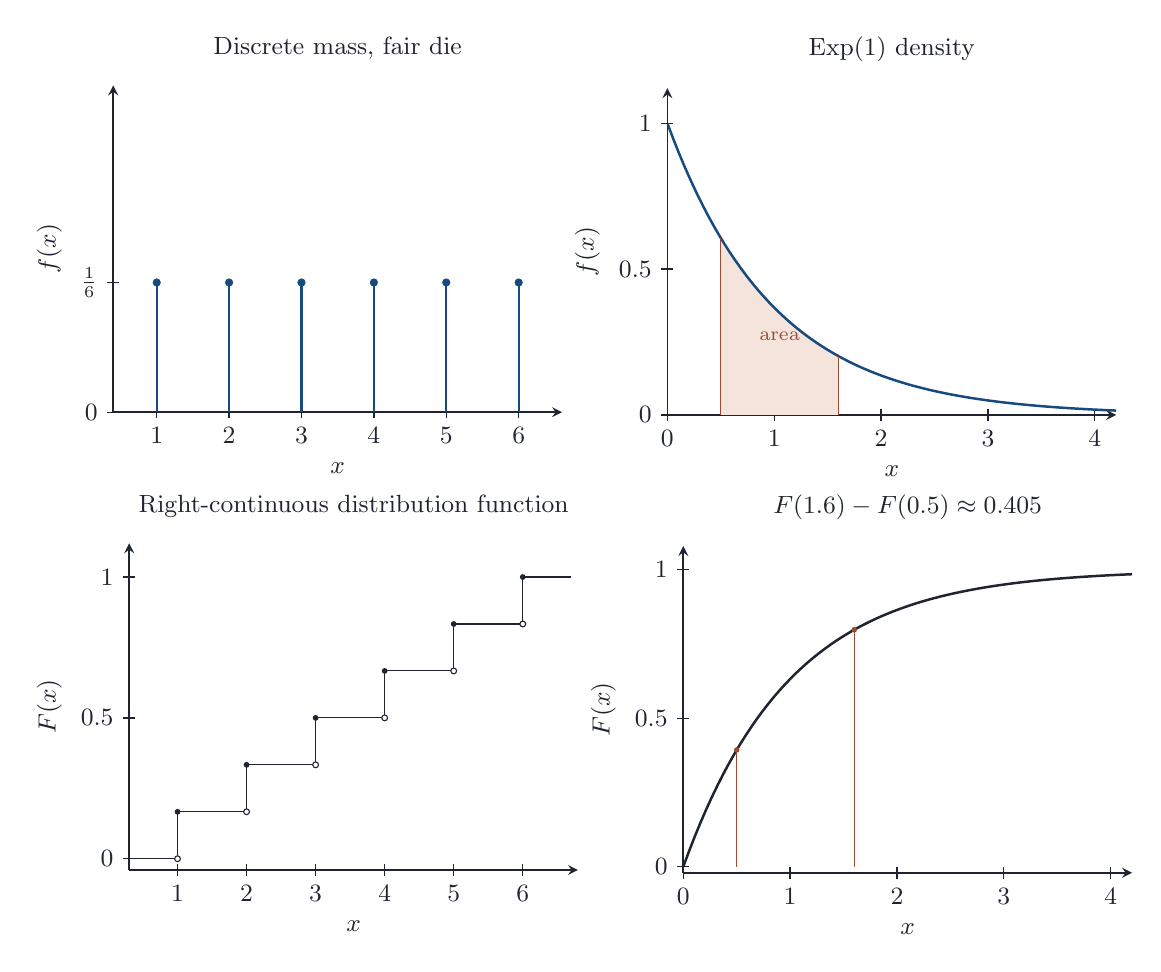
\begin{tikzpicture}
\begin{axis}[
  stat, name=pmf, width=5.7cm, height=4.15cm,
  xmin=0.4, xmax=6.6, ymin=0, ymax=0.42,
  xtick={1,2,3,4,5,6},
  ytick={0,0.1666667},
  yticklabels={$0$,$\tfrac{1}{6}$},
  xlabel={$x$},
  ylabel={$f(x)$},
  title={Discrete mass, fair die},
]
  \addplot[ycomb, statblue, mark=*, mark size=1.05pt, line width=0.8pt, forget plot] coordinates {
    (1,0.166667) (2,0.166667) (3,0.166667) (4,0.166667) (5,0.166667) (6,0.166667)
  };
\end{axis}

\begin{axis}[
  stat, name=den, width=5.7cm, height=4.15cm,
  at={($(pmf.outer north east)+(1.05,0)$)}, anchor=outer north west,
  xmin=0, xmax=4.2, ymin=0, ymax=1.12,
  xtick={0,1,2,3,4},
  ytick={0,0.5,1},
  xlabel={$x$},
  ylabel={$f(x)$},
  title={$\operatorname{Exp}(1)$ density},
]
  \addplot[name path=dens, statblue, line width=0.9pt, domain=0:4.2, samples=80] {exp(-x)};
  \addplot[name path=zero, draw=none, domain=0:4.2] {0};
  \addplot[accentfill] fill between[of=dens and zero, soft clip={domain=0.5:1.6}];
  \draw[accent, thin] (axis cs:0.5,0) -- (axis cs:0.5,{exp(-0.5)});
  \draw[accent, thin] (axis cs:1.6,0) -- (axis cs:1.6,{exp(-1.6)});
  \node[font=\scriptsize, accent, anchor=south] at (axis cs:1.05,0.22) {area};
\end{axis}

\begin{axis}[
  stat, name=dcdf, width=5.7cm, height=4.15cm,
  at={($(pmf.outer south west)+(0,-0.95)$)}, anchor=outer north west,
  xmin=0.3, xmax=6.8, ymin=-0.04, ymax=1.12,
  xtick={1,2,3,4,5,6},
  ytick={0,0.5,1},
  xlabel={$x$},
  ylabel={$F(x)$},
  title={Right-continuous distribution function},
]
  \draw[ink, thin]
    (axis cs:0.35,0) -- (axis cs:1,0) -- (axis cs:1,0.166667) -- (axis cs:2,0.166667)
    -- (axis cs:2,0.333333) -- (axis cs:3,0.333333)
    -- (axis cs:3,0.5) -- (axis cs:4,0.5)
    -- (axis cs:4,0.666667) -- (axis cs:5,0.666667)
    -- (axis cs:5,0.833333) -- (axis cs:6,0.833333)
    -- (axis cs:6,1) -- (axis cs:6.7,1);
  \fill[white, draw=ink, thin] (axis cs:1,0) circle[radius=1.05pt];
  \fill[white, draw=ink, thin] (axis cs:2,0.166667) circle[radius=1.05pt];
  \fill[white, draw=ink, thin] (axis cs:3,0.333333) circle[radius=1.05pt];
  \fill[white, draw=ink, thin] (axis cs:4,0.5) circle[radius=1.05pt];
  \fill[white, draw=ink, thin] (axis cs:5,0.666667) circle[radius=1.05pt];
  \fill[white, draw=ink, thin] (axis cs:6,0.833333) circle[radius=1.05pt];
  \fill[ink] (axis cs:1,0.166667) circle[radius=1.05pt];
  \fill[ink] (axis cs:2,0.333333) circle[radius=1.05pt];
  \fill[ink] (axis cs:3,0.5) circle[radius=1.05pt];
  \fill[ink] (axis cs:4,0.666667) circle[radius=1.05pt];
  \fill[ink] (axis cs:5,0.833333) circle[radius=1.05pt];
  \fill[ink] (axis cs:6,1) circle[radius=1.05pt];
\end{axis}

\begin{axis}[
  stat, width=5.7cm, height=4.15cm,
  at={($(dcdf.outer north east)+(1.05,0)$)}, anchor=outer north west,
  xmin=0, xmax=4.2, ymin=-0.02, ymax=1.08,
  xtick={0,1,2,3,4},
  ytick={0,0.5,1},
  xlabel={$x$},
  ylabel={$F(x)$},
  title={$F(1.6)-F(0.5)\approx 0.405$},
]
  \addplot[ink, line width=0.9pt, domain=0:4.2, samples=80] {1-exp(-x)};
  \draw[accent, thin] (axis cs:0.5,0) -- (axis cs:0.5,0.393469);
  \draw[accent, thin] (axis cs:1.6,0) -- (axis cs:1.6,0.798103);
  \draw[accent, thin] (axis cs:1.6,0.393469) -- (axis cs:1.6,0.798103);
  \fill[accent] (axis cs:0.5,0.393469) circle[radius=1.0pt];
  \fill[accent] (axis cs:1.6,0.798103) circle[radius=1.0pt];
\end{axis}
\end{tikzpicture}
\end{document}
